\documentclass[12pt,a4paper]{article}

\usepackage{fontspec}
\usepackage[brazil]{babel}
\usepackage[margin=2.5cm]{geometry}
\usepackage{graphicx}
\usepackage{float}
\usepackage{amsmath}
\usepackage{xcolor}
\usepackage{listings}
\usepackage{caption}
\usepackage{hyperref}
\hypersetup{hidelinks}

% ---------- estilo das listagens de codigo MATLAB ----------
\lstdefinestyle{mat}{
  language=Matlab,
  basicstyle=\ttfamily\footnotesize,
  keywordstyle=\color{blue},
  commentstyle=\color{teal},
  stringstyle=\color{magenta},
  numbers=left,
  numberstyle=\tiny\color{gray},
  numbersep=7pt,
  frame=single,
  rulecolor=\color{gray!55},
  breaklines=true,
  showstringspaces=false,
  tabsize=2,
  columns=fullflexible,
  upquote=true,
  aboveskip=10pt, belowskip=10pt,
}
\lstset{style=mat}
\captionsetup{font=small}

\begin{document}

% ============================ CAPA ============================
\begin{titlepage}
\centering
{\Large\bfseries UNIVERSIDADE TECNOL\'OGICA FEDERAL DO PARAN\'A\par}
{\Large\bfseries CURSO DE ENGENHARIA DE COMPUTA\c{C}\~AO\par}
\vspace{0.4cm}
{ELEQ30 - An\'alise de Sistemas Lineares\par}
{Professor C\'esar Janeczko\par}

\vspace{4.5cm}
{\Huge\bfseries Relat\'orio: Pr\'atica 5\par}
\vspace{0.4cm}
{\large\bfseries Filtros IIR (Filtros Recursivos) - Som\par}

\vspace{2.5cm}
{\large\bfseries Disciplina: An\'alise de Sistemas Lineares\par}

\vspace{3.5cm}
{Leonardo Pereira Shibata\par}
\vspace{0.2cm}
{Sergio Roncato Maccari\par}

\vfill
{Curitiba, Junho de 2026\par}
\end{titlepage}

% ============================ ITEM 1 ============================
\section{Filtros de p\'olo simples (R-C): passa-baixas e passa-altas}
\textbf{Enunciado:} ``Implemente rotina MATLAB para calcular coeficientes de
filtros de P\'olo simples (R-C) passa-baixas e passa-altas. Voc\^e escolhe fc.
Encontre os gr\'aficos da resposta ao impulso (1 0 0 0 0 0  0....(100 pontos)) e
das respostas em frequ\^encia (ganho, atenua\c{c}\~ao e fase).''

\vspace{0.3cm}
O filtro passa-baixas de p\'olo simples \'e o equivalente discreto de um circuito
R-C. A partir da frequ\^encia de corte normalizada $f_c$ define-se a constante
$r = e^{-2\pi f_c}$, que posiciona o \'unico p\'olo do sistema. Quanto mais
pr\'oximo de $1$ for $r$, mais lenta \'e a resposta ao impulso e menor \'e a
frequ\^encia de corte. A equa\c{c}\~ao de diferen\c{c}as \'e
$y[n] = a_0\,x[n] + b_1\,y[n-1]$, com $a_0 = 1-r$ e $b_1 = r$, garantindo ganho
unit\'ario em corrente cont\'inua. Escolheu-se $f_c = 0{,}10$.

\lstinputlisting[caption={Filtro passa-baixas IIR de p\'olo simples.}]{codigo_matlab/CalculaFPBIIR.m}

\begin{figure}[H]
\centering
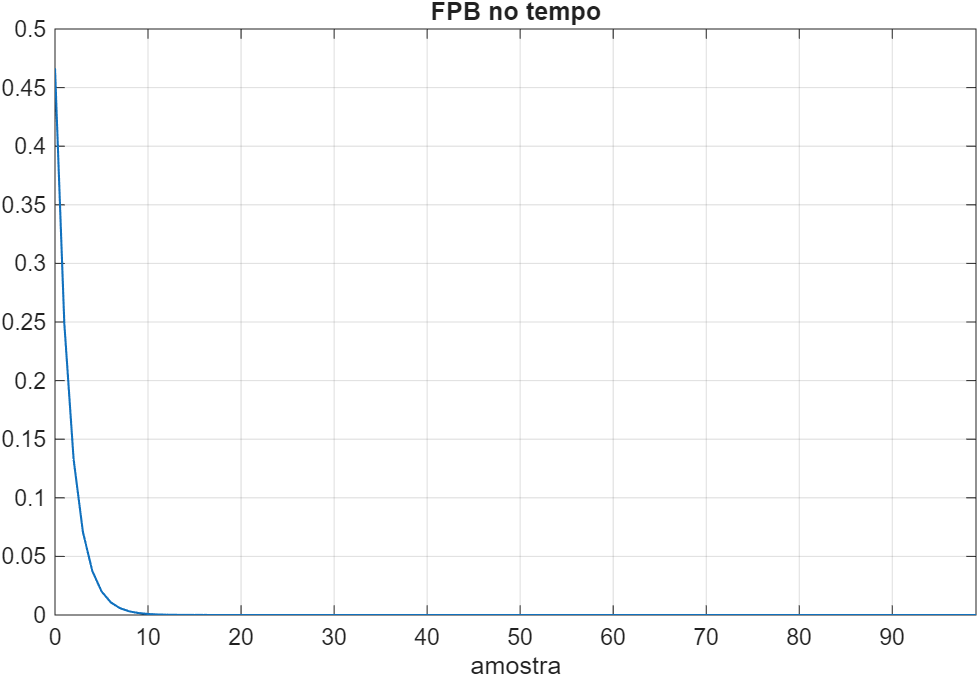
\includegraphics[width=0.8\linewidth]{figs/f1_fpb_tempo.png}
\caption{Resposta ao impulso do FPB de p\'olo simples no tempo ($f_c=0{,}10$),
calculada sobre 100 pontos.}
\end{figure}

\begin{figure}[H]
\centering
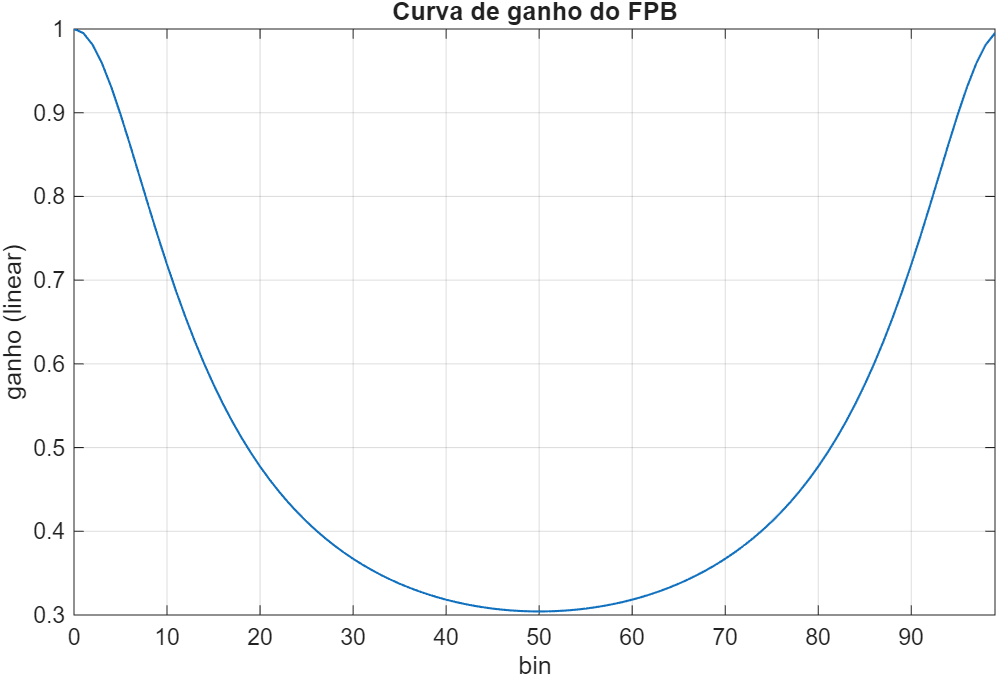
\includegraphics[width=0.8\linewidth]{figs/f1_fpb_ganho.png}
\caption{Curva de ganho (linear) do FPB de p\'olo simples ($f_c=0{,}10$).}
\end{figure}

\begin{figure}[H]
\centering
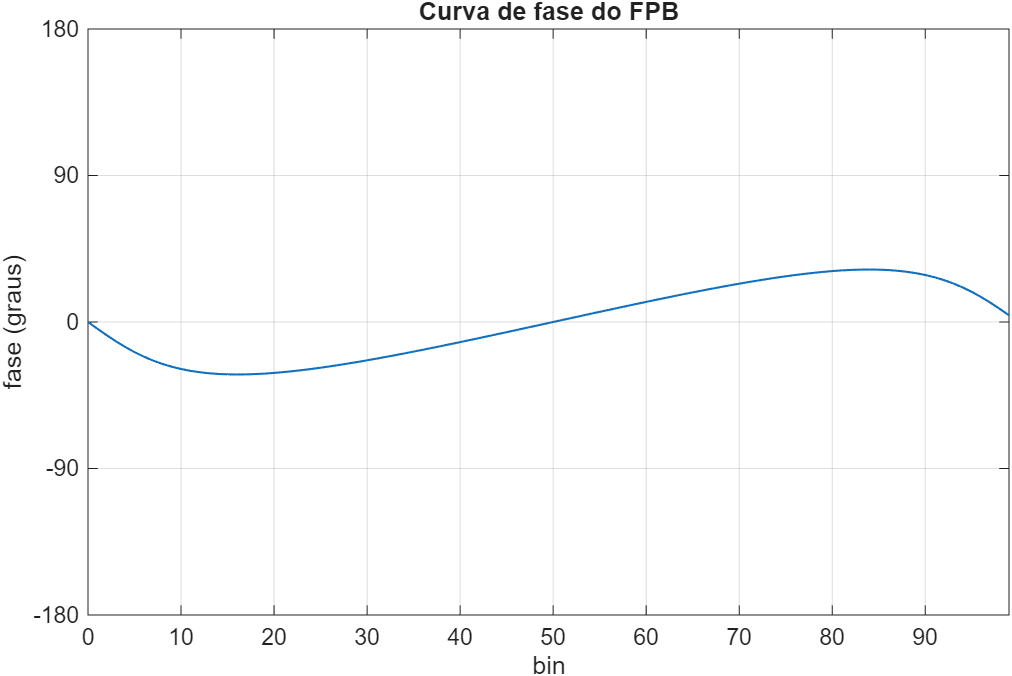
\includegraphics[width=0.8\linewidth]{figs/f1_fpb_fase.png}
\caption{Curva de fase (em graus) do FPB de p\'olo simples ($f_c=0{,}10$).}
\end{figure}

A resposta ao impulso decai exponencialmente, como esperado de um sistema de
primeira ordem. A curva de ganho parte de $1$ em corrente cont\'inua e cai
suavemente at\'e a frequ\^encia de Nyquist (\'indice 50), evidenciando a transi\c{c}\~ao
gradual t\'ipica de um \'unico p\'olo. A simetria em torno do \'indice 50 decorre
da FFT de um sinal real.

\vspace{0.3cm}
O passa-altas \'e obtido pela vers\~ao complementar do mesmo p\'olo: mant\'em-se
$b_1 = r$ e usam-se $a_0 = (1+r)/2$ e $a_1 = -(1+r)/2$, de modo que a componente
cont\'inua \'e cancelada e as altas frequ\^encias s\~ao preservadas.

\lstinputlisting[caption={Filtro passa-altas IIR de p\'olo simples.}]{codigo_matlab/CalculaFPAIIR.m}

\begin{figure}[H]
\centering
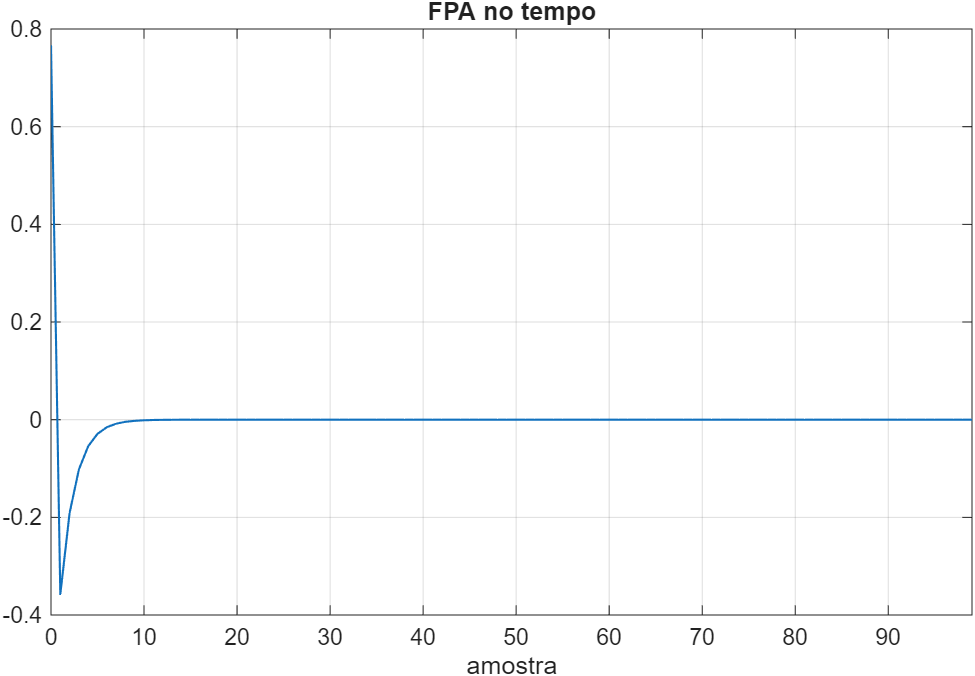
\includegraphics[width=0.8\linewidth]{figs/f1_fpa_tempo.png}
\caption{Resposta ao impulso do FPA de p\'olo simples no tempo ($f_c=0{,}10$).}
\end{figure}

\begin{figure}[H]
\centering
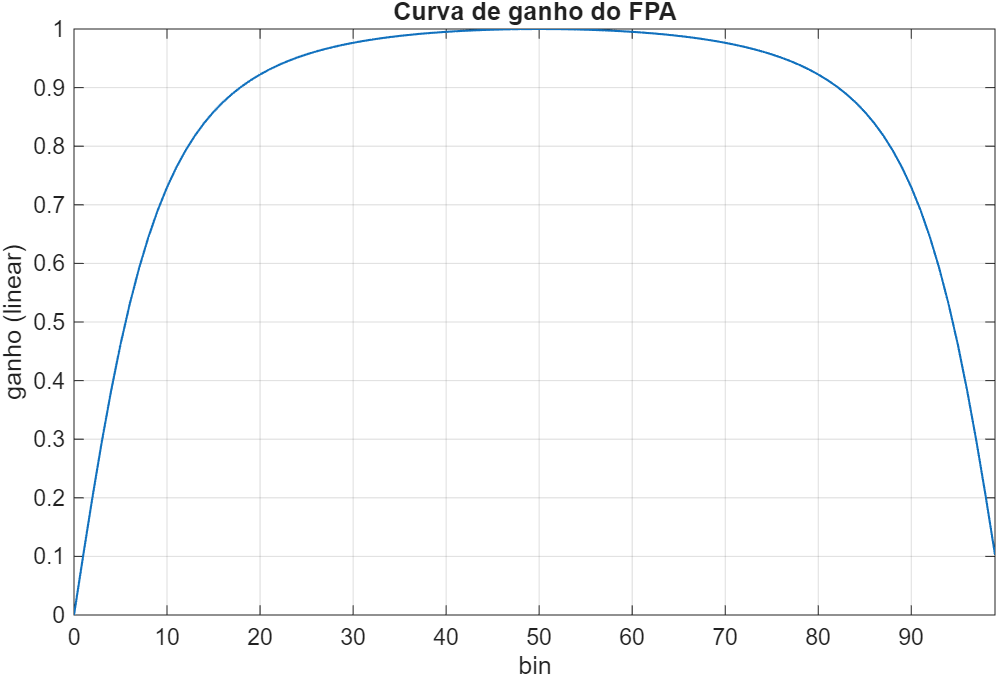
\includegraphics[width=0.8\linewidth]{figs/f1_fpa_ganho.png}
\caption{Curva de ganho (linear) do FPA de p\'olo simples ($f_c=0{,}10$).}
\end{figure}

\begin{figure}[H]
\centering
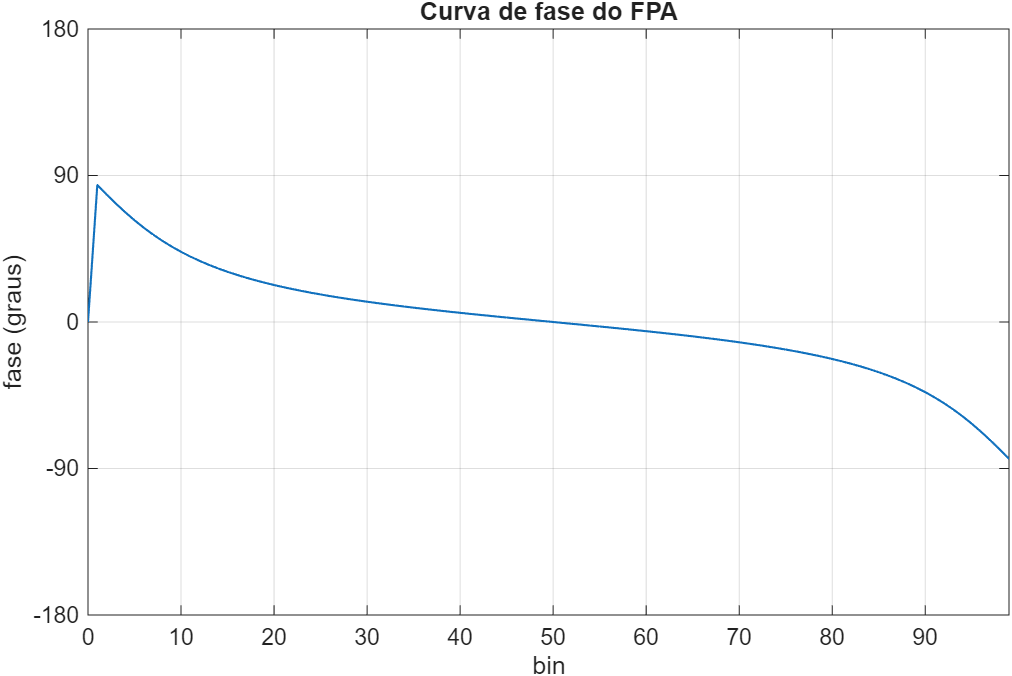
\includegraphics[width=0.8\linewidth]{figs/f1_fpa_fase.png}
\caption{Curva de fase (em graus) do FPA de p\'olo simples ($f_c=0{,}10$).}
\end{figure}

No FPA o ganho \'e praticamente nulo em corrente cont\'inua e cresce em dire\c{c}\~ao
\`as altas frequ\^encias, comportamento oposto ao do FPB. Por ser de primeira
ordem, a transi\c{c}\~ao tamb\'em \'e suave.

% ============================ ITEM 2 ============================
\section{Teste dos filtros FPB e FPA}
\textbf{Enunciado:} ``Elabore um sinal com baixa frequ\^encia + alta frequ\^encia
e teste os filtros FPB e FPA calculados com as rotinas anteriores do item 1).
Mostre o sinal gerado e os sinais filtrados (no tempo e na frequ\^encia).''

\vspace{0.3cm}
Gerou-se um sinal com 1000 amostras ($F_s = 1000$~Hz) somando uma componente de
baixa frequ\^encia (30~Hz) e uma de alta frequ\^encia (350~Hz):
$x[n] = \operatorname{sen}(2\pi\,30\,n/1000) + \operatorname{sen}(2\pi\,350\,n/1000)$.

\begin{figure}[H]
\centering
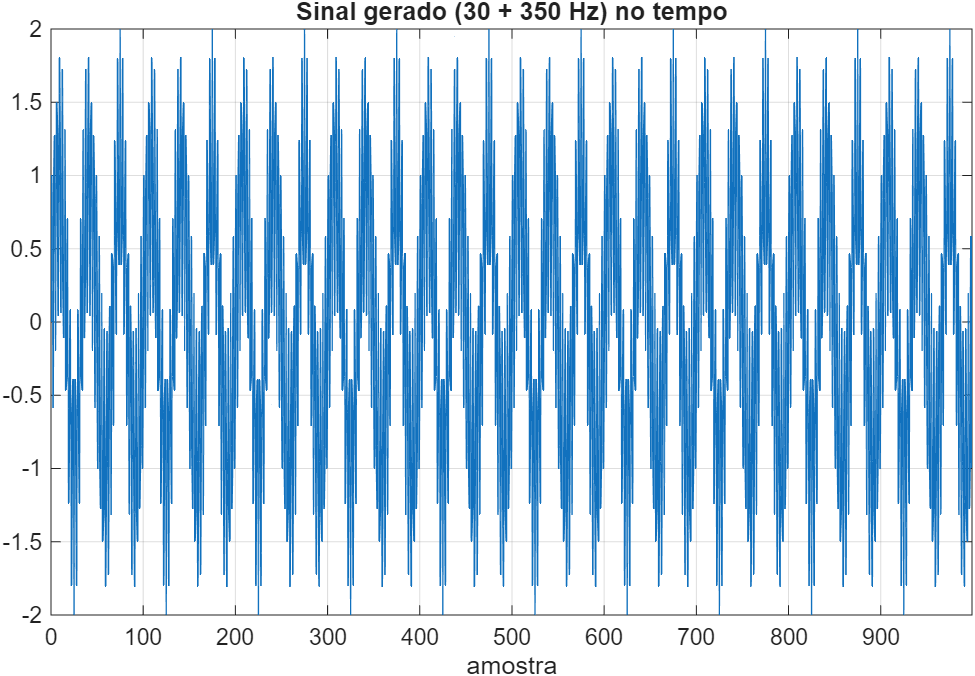
\includegraphics[width=0.8\linewidth]{figs/f2_sinal_tempo.png}
\caption{Sinal gerado (30~Hz + 350~Hz) no tempo.}
\end{figure}

\begin{figure}[H]
\centering
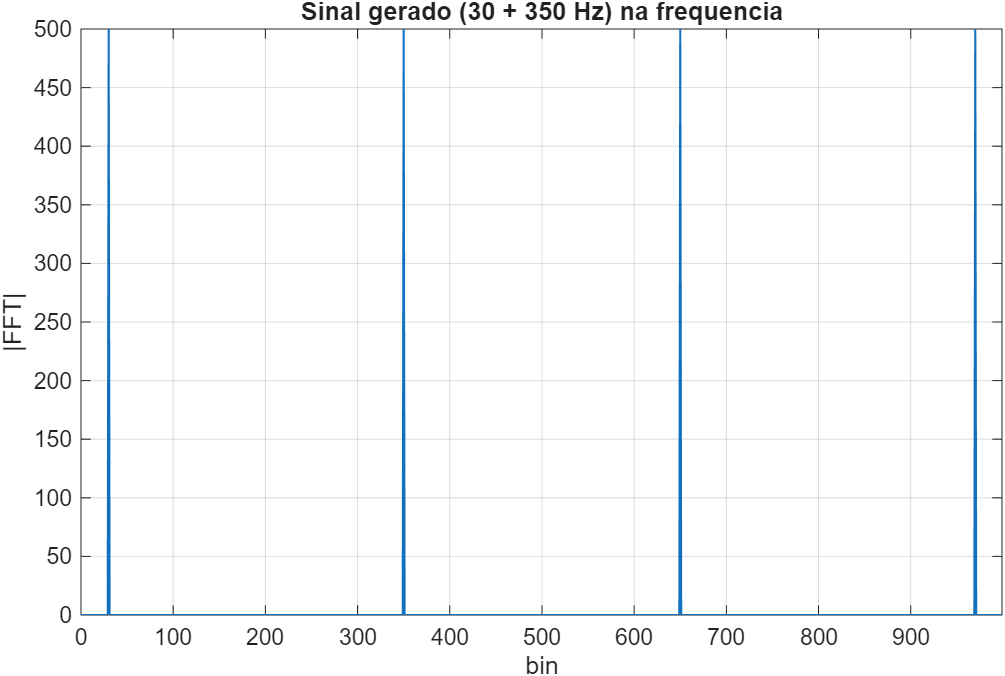
\includegraphics[width=0.8\linewidth]{figs/f2_sinal_freq.png}
\caption{Sinal gerado (30~Hz + 350~Hz) na frequ\^encia. As raias aparecem em 30 e
350~Hz, com os espelhos em torno dos \'indices 650 e 970 (espelhamento da FFT em
torno de $F_s/2$).}
\end{figure}

\begin{figure}[H]
\centering
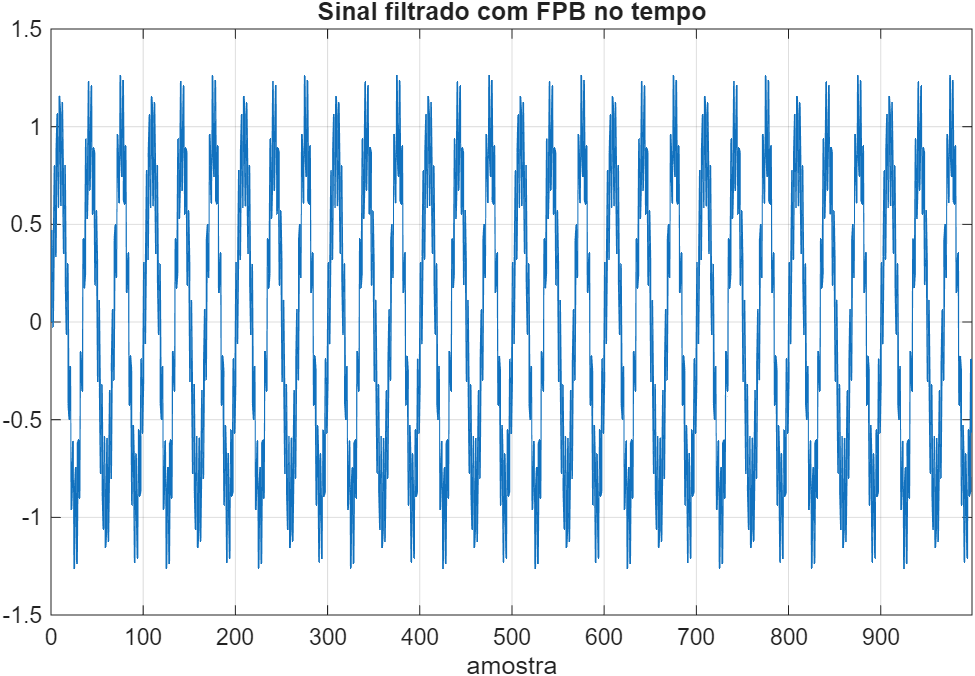
\includegraphics[width=0.8\linewidth]{figs/f2_fpb_tempo.png}
\caption{Sinal filtrado com o FPB no tempo.}
\end{figure}

\begin{figure}[H]
\centering
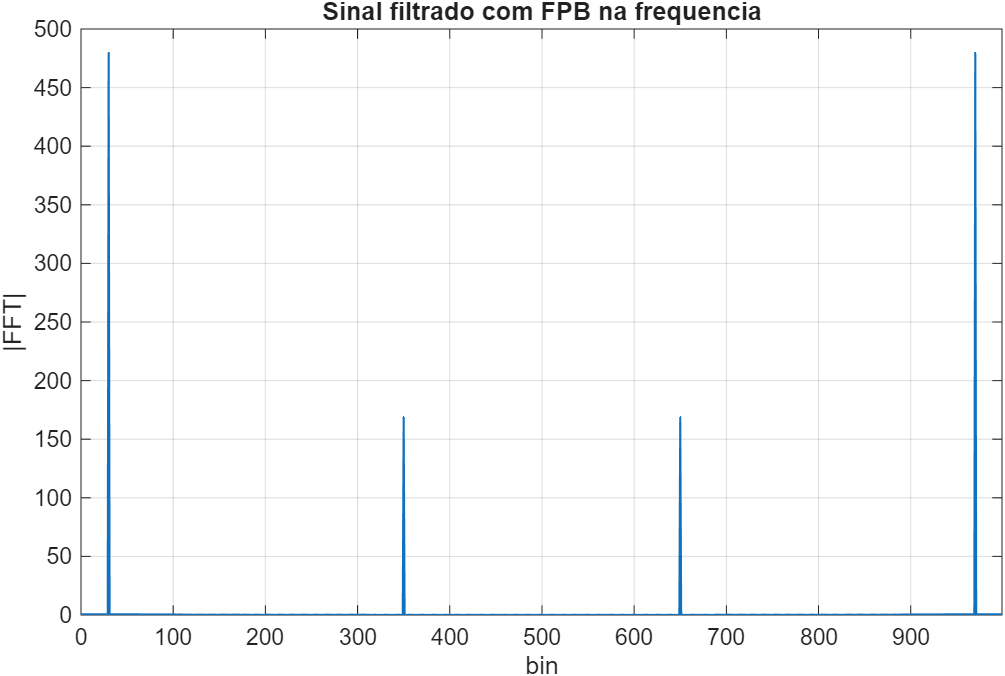
\includegraphics[width=0.8\linewidth]{figs/f2_fpb_freq.png}
\caption{Sinal filtrado com o FPB na frequ\^encia: a raia de 30~Hz \'e preservada
e a de 350~Hz \'e atenuada.}
\end{figure}

\begin{figure}[H]
\centering
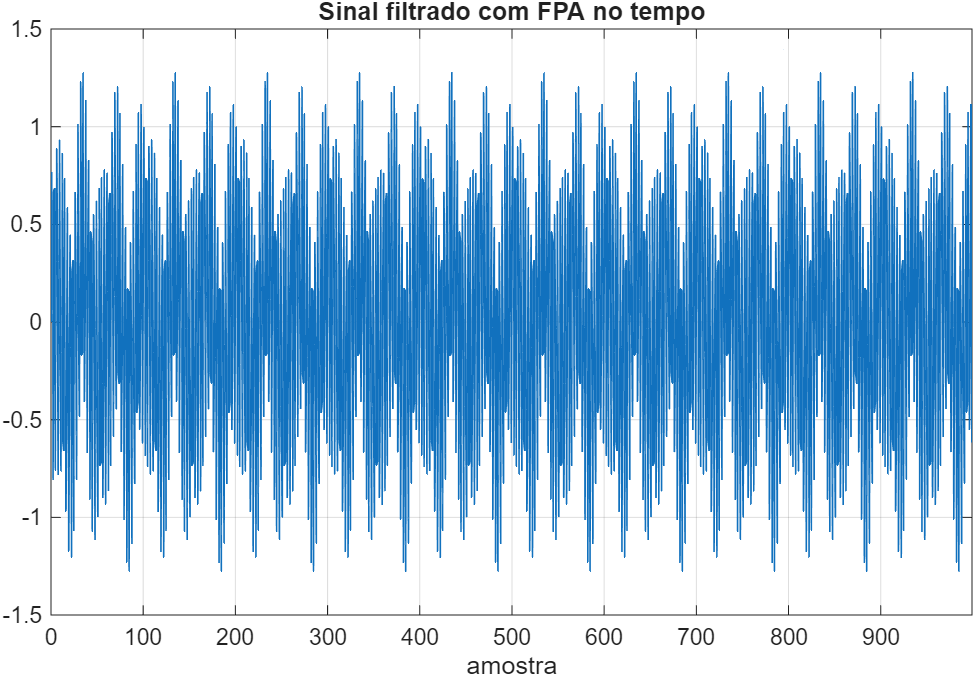
\includegraphics[width=0.8\linewidth]{figs/f2_fpa_tempo.png}
\caption{Sinal filtrado com o FPA no tempo.}
\end{figure}

\begin{figure}[H]
\centering
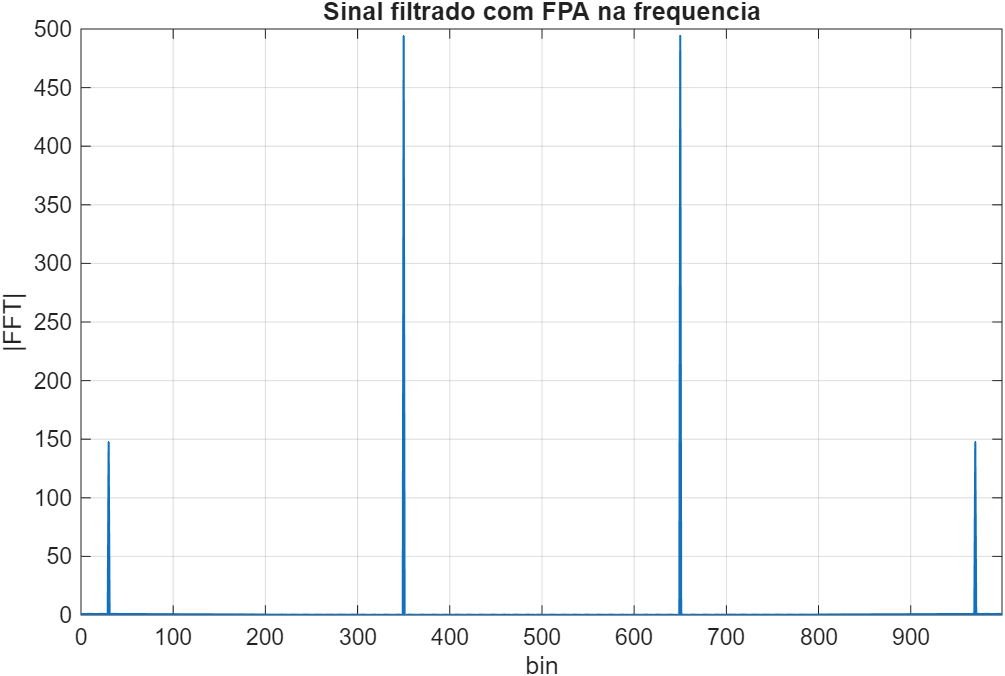
\includegraphics[width=0.8\linewidth]{figs/f2_fpa_freq.png}
\caption{Sinal filtrado com o FPA na frequ\^encia: a raia de 350~Hz \'e preservada
e a de 30~Hz \'e atenuada.}
\end{figure}

No espectro do sinal gerado aparecem as raias em 30 e 350~Hz (e seus espelhos).
Ap\'os o FPB, a raia de 30~Hz \'e preservada e a de 350~Hz \'e fortemente
atenuada; ap\'os o FPA ocorre o inverso. Como os filtros s\~ao de p\'olo simples,
a atenua\c{c}\~ao da componente indesejada \'e parcial (n\~ao h\'a corte abrupto),
o que \'e coerente com as curvas de ganho do item~1.

% ============================ ITEM 3 ============================
\section{Filtros de banda estreita: passa-banda e rejeita-banda}
\textbf{Enunciado:} ``Implemente rotina MATLAB para calcular coeficientes de
filtros Banda estreita (passa-banda e corta-banda). Voc\^e escolhe fc e BW.
OBS: BW dever ser estreito! Encontre os gr\'aficos da resposta ao impulso
(1 0 0 0 0 0  0....(100 pontos)) e das respostas em frequ\^encia (ganho,
atenua\c{c}\~ao e fase).''

\vspace{0.3cm}
Os filtros de banda estreita s\~ao sistemas recursivos de segunda ordem
(resonadores). A largura de banda $BW$ define a posi\c{c}\~ao dos p\'olos por meio
de $r = 1 - 3\,BW$ (quanto menor o $BW$, mais pr\'oximo de $1$ fica $r$ e mais
estreita \'e a banda). O fator de normaliza\c{c}\~ao \'e
\[
K = \frac{1 - 2r\cos(2\pi f) + r^{2}}{2 - 2\cos(2\pi f)} .
\]
Escolheu-se a frequ\^encia central $f_c = 0{,}25$ e $BW = 0{,}008$ (banda
estreita).

\lstinputlisting[caption={Filtro recursivo passa-banda de banda estreita.}]{codigo_matlab/FiltroPassaBanda.m}

\begin{figure}[H]
\centering
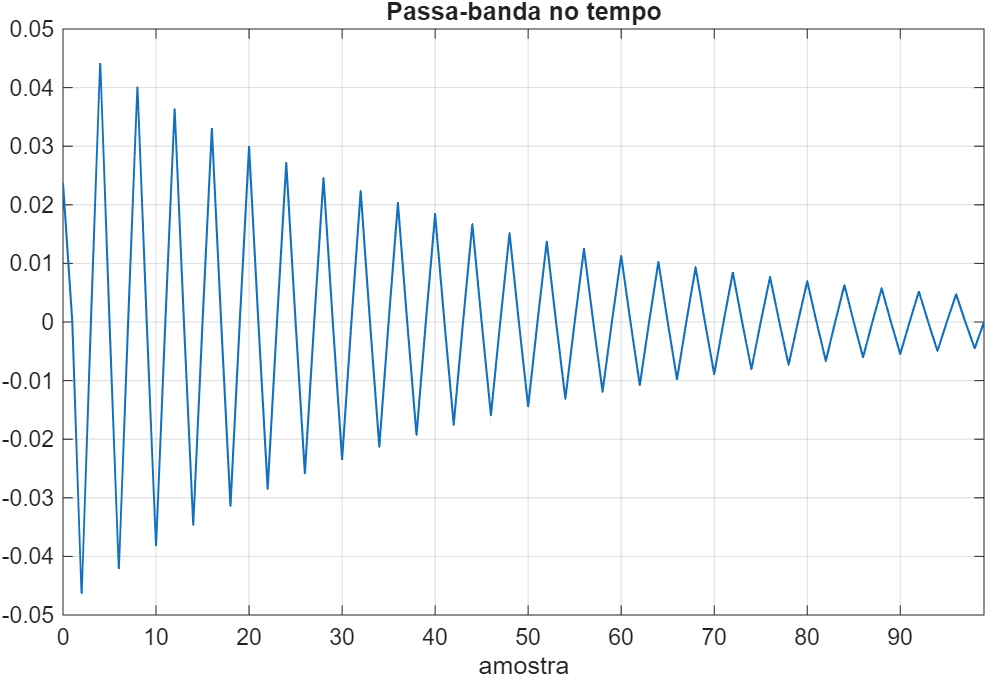
\includegraphics[width=0.8\linewidth]{figs/f3_bp_tempo.png}
\caption{Resposta ao impulso do passa-banda no tempo (senoide amortecida)
($f_c=0{,}25$, $BW=0{,}008$).}
\end{figure}

\begin{figure}[H]
\centering
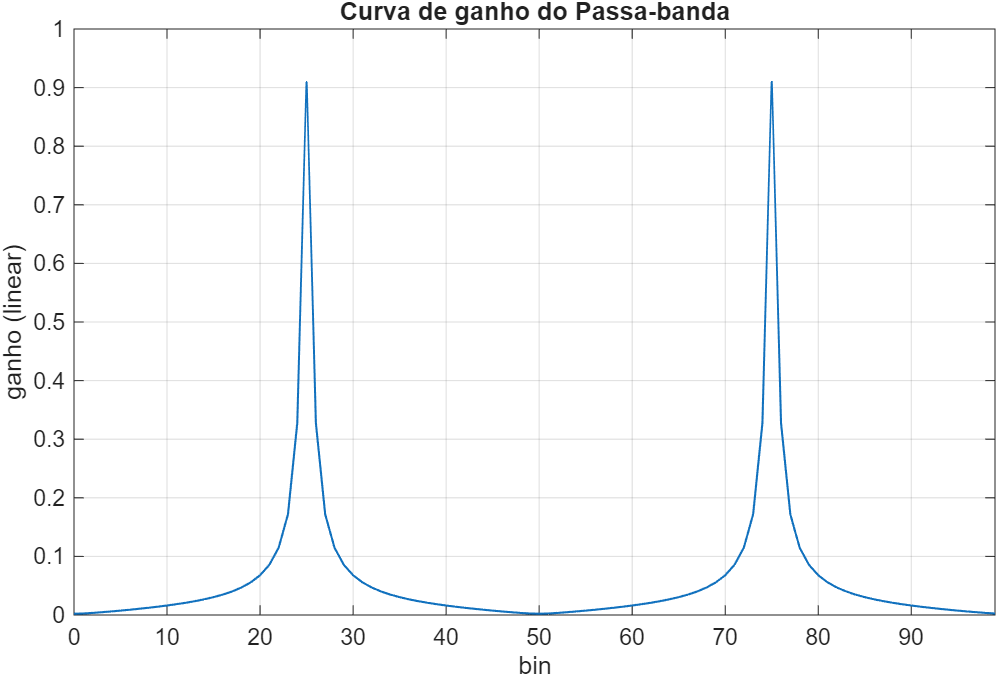
\includegraphics[width=0.8\linewidth]{figs/f3_bp_ganho.png}
\caption{Curva de ganho (linear) do passa-banda ($f_c=0{,}25$, $BW=0{,}008$).}
\end{figure}

\begin{figure}[H]
\centering
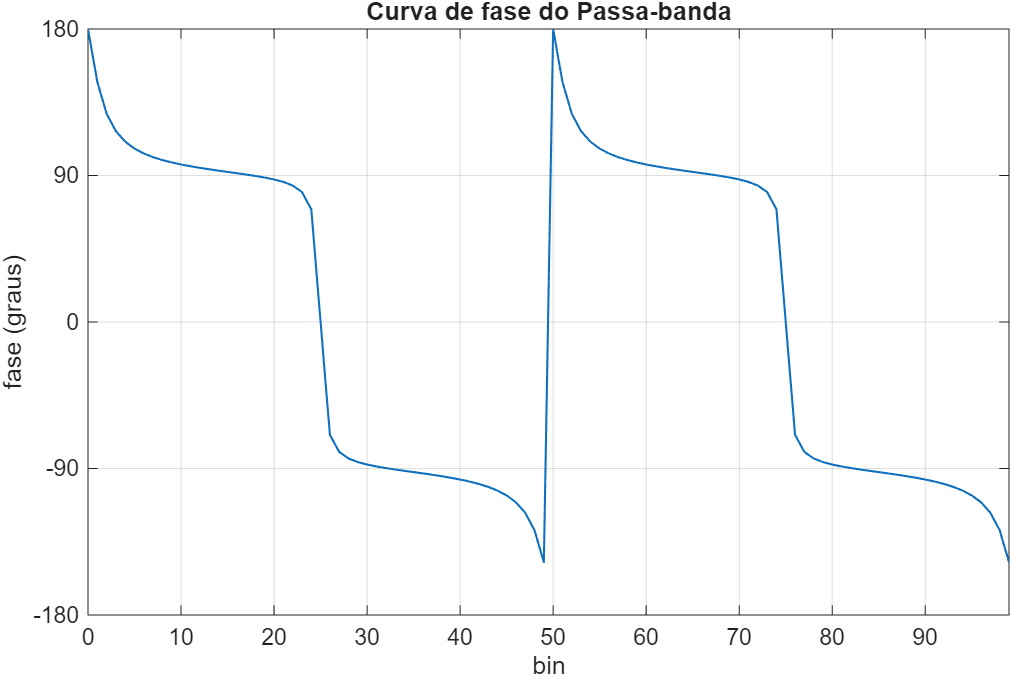
\includegraphics[width=0.8\linewidth]{figs/f3_bp_fase.png}
\caption{Curva de fase (em graus) do passa-banda ($f_c=0{,}25$, $BW=0{,}008$).}
\end{figure}

\lstinputlisting[caption={Filtro recursivo rejeita-banda (notch) de banda estreita.}]{codigo_matlab/FiltroRejeitaBanda.m}

\begin{figure}[H]
\centering
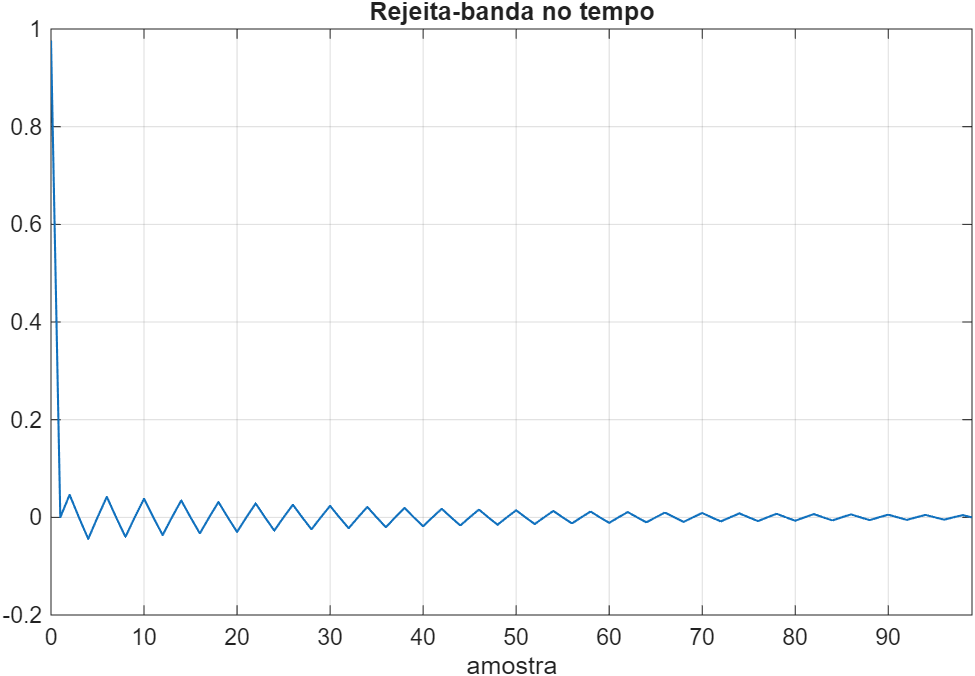
\includegraphics[width=0.8\linewidth]{figs/f3_br_tempo.png}
\caption{Resposta ao impulso do rejeita-banda no tempo ($f_c=0{,}25$,
$BW=0{,}008$).}
\end{figure}

\begin{figure}[H]
\centering
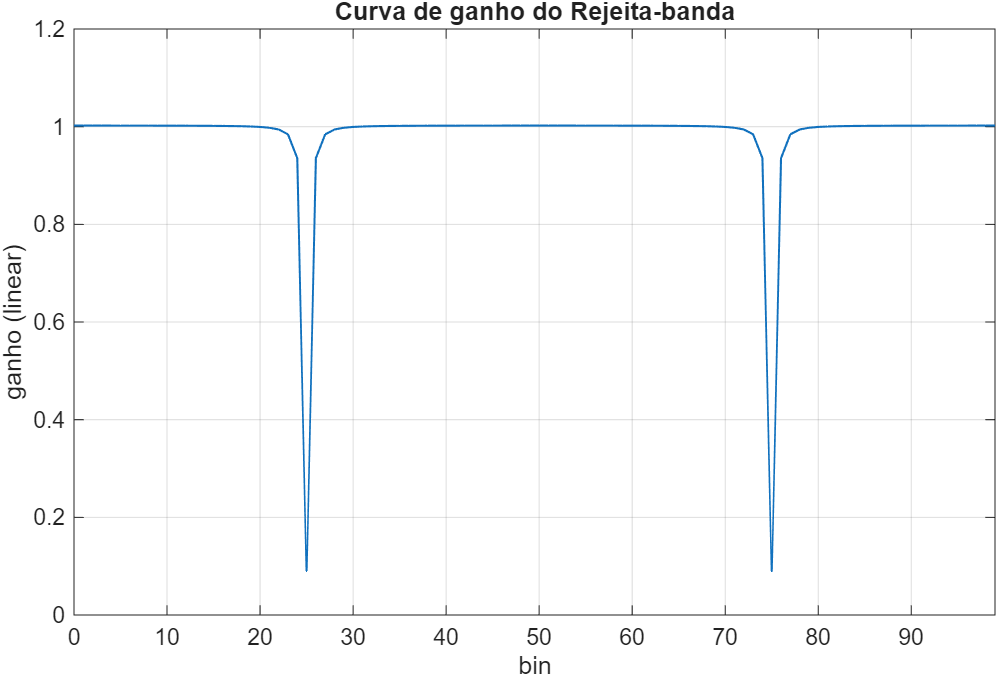
\includegraphics[width=0.8\linewidth]{figs/f3_br_ganho.png}
\caption{Curva de ganho (linear) do rejeita-banda ($f_c=0{,}25$, $BW=0{,}008$).}
\end{figure}

\begin{figure}[H]
\centering
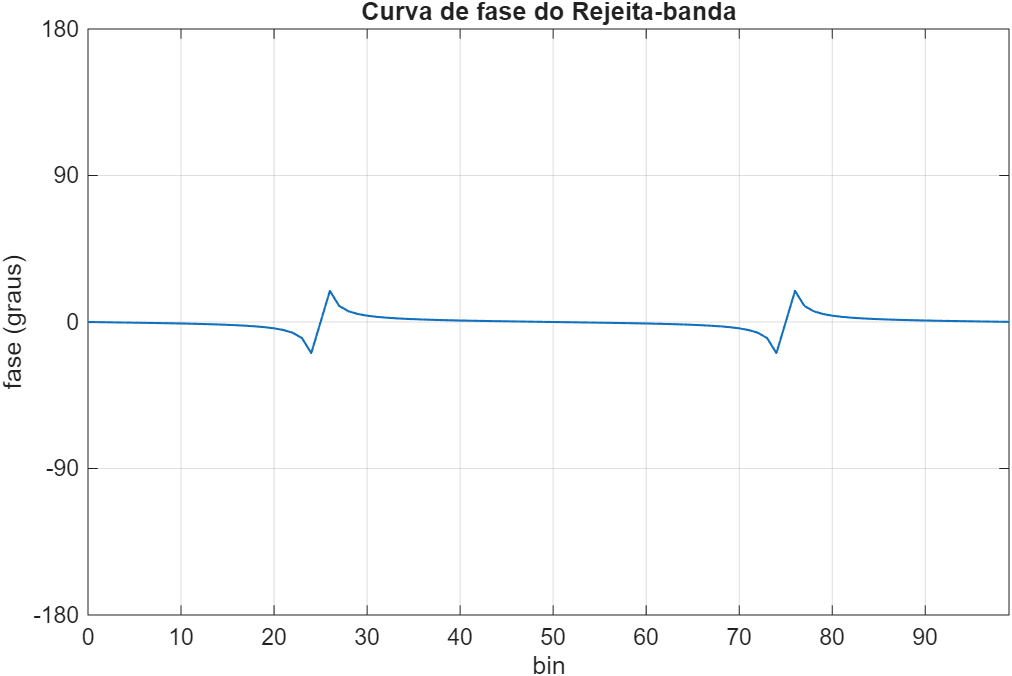
\includegraphics[width=0.8\linewidth]{figs/f3_br_fase.png}
\caption{Curva de fase (em graus) do rejeita-banda ($f_c=0{,}25$, $BW=0{,}008$).}
\end{figure}

A resposta ao impulso do passa-banda \'e uma senoide amortecida, cuja taxa de
decaimento depende de $r$. No dom\'inio da frequ\^encia, o passa-banda apresenta
um pico estreito no \'indice 25 (e o espelho no \'indice 75), enquanto o
rejeita-banda apresenta um entalhe profundo exatamente nessas posi\c{c}\~oes,
mantendo ganho unit\'ario no restante do espectro.

% ============================ ITEM 4 ============================
\section{Teste dos filtros de banda estreita}
\textbf{Enunciado:} ``Elabore um sinal com v\'arias frequ\^encias a sua escola,
sinal este que seja compat\'ivel com as frequ\^encias de corte dos filtros
implementados no item 3). Teste os filtros passa-banda e corta-banda, banda
estreita, calculados com a rotina anterior, item 3). Mostre o sinal gerado e os
sinais filtrados (no tempo e na frequ\^encia).''

\vspace{0.3cm}
Gerou-se um sinal com cinco senoides ($F_s=1000$~Hz): 40, 120, 250, 380 e
470~Hz. A componente de 250~Hz coincide com a frequ\^encia central dos filtros
($f_c=0{,}25 \Rightarrow 250$~Hz), permitindo demonstrar o isolamento e a
rejei\c{c}\~ao seletivos.

\begin{figure}[H]
\centering
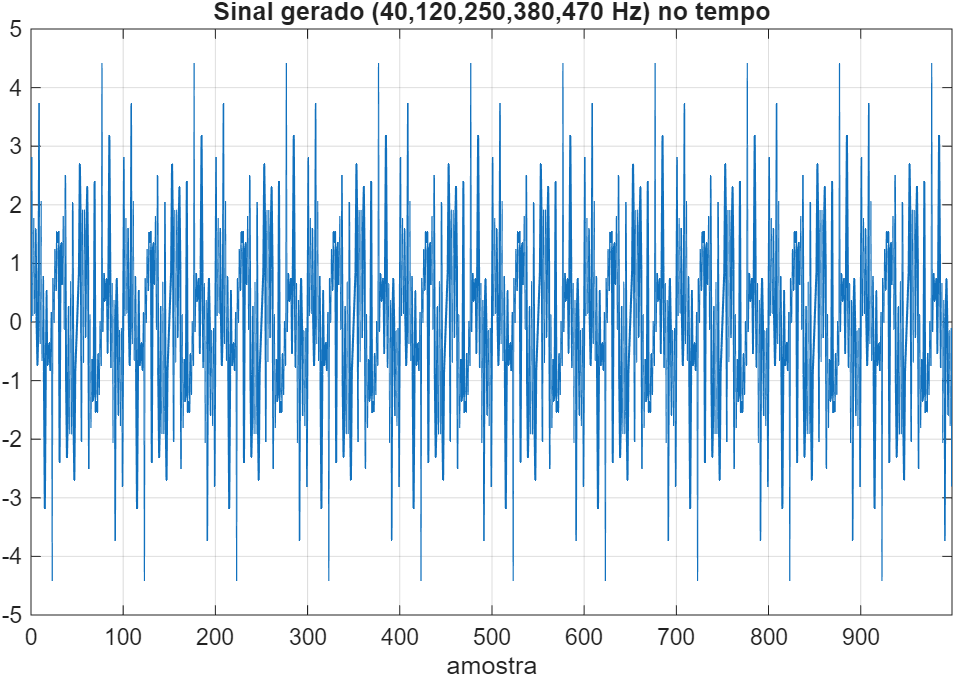
\includegraphics[width=0.8\linewidth]{figs/f4_sinal_tempo.png}
\caption{Sinal gerado (40, 120, 250, 380 e 470~Hz) no tempo.}
\end{figure}

\begin{figure}[H]
\centering
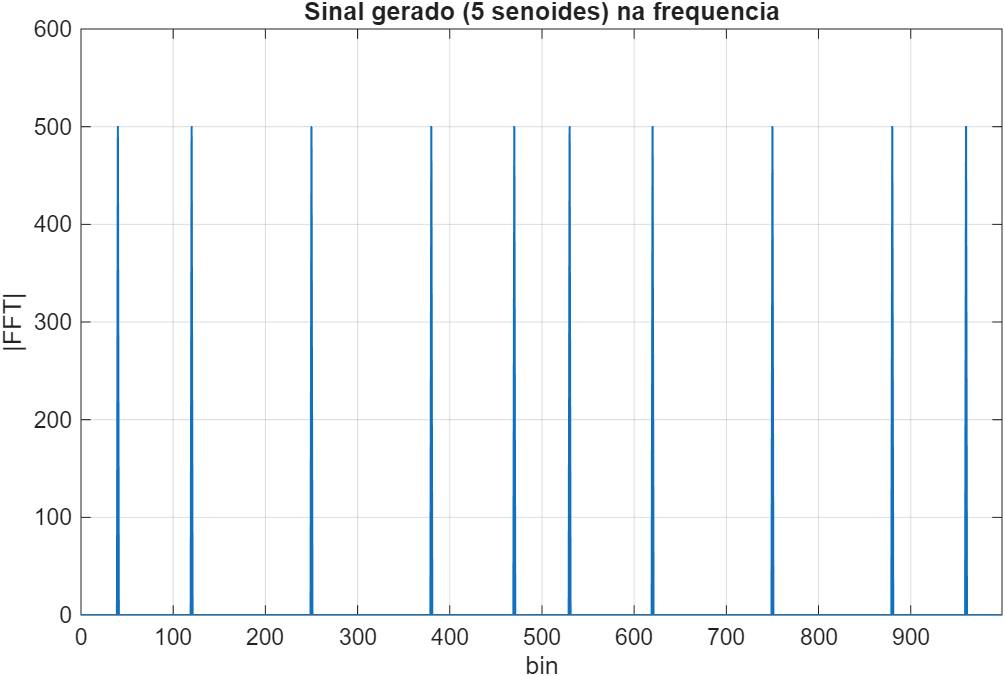
\includegraphics[width=0.8\linewidth]{figs/f4_sinal_freq.png}
\caption{Sinal gerado (cinco senoides) na frequ\^encia: raias em 40, 120, 250, 380
e 470~Hz (e seus espelhos).}
\end{figure}

\begin{figure}[H]
\centering
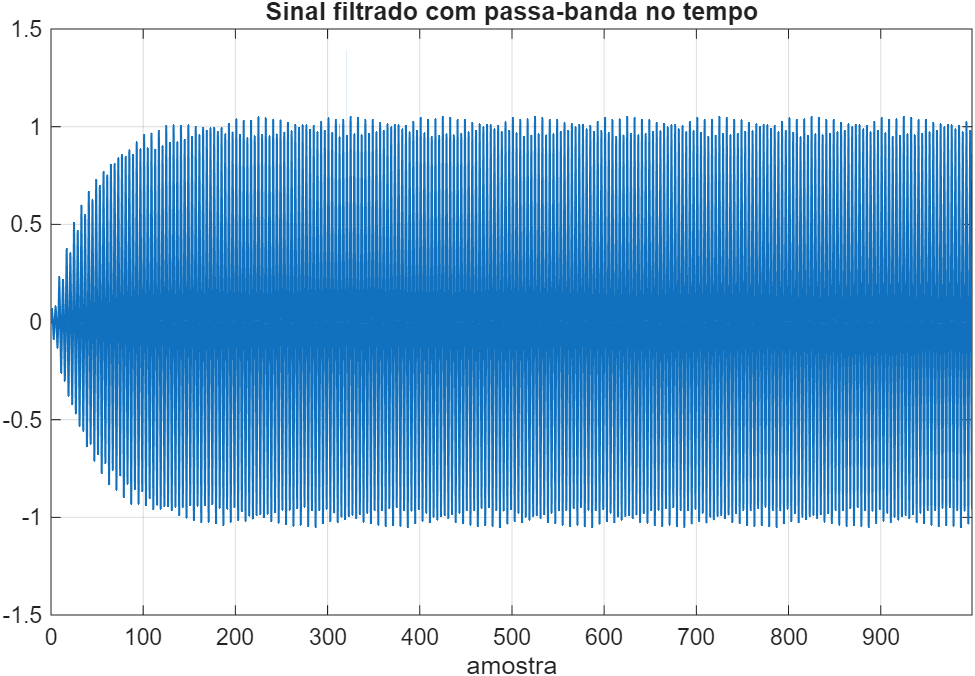
\includegraphics[width=0.8\linewidth]{figs/f4_bp_tempo.png}
\caption{Sinal filtrado com o passa-banda (centrado em 250~Hz) no tempo.}
\end{figure}

\begin{figure}[H]
\centering
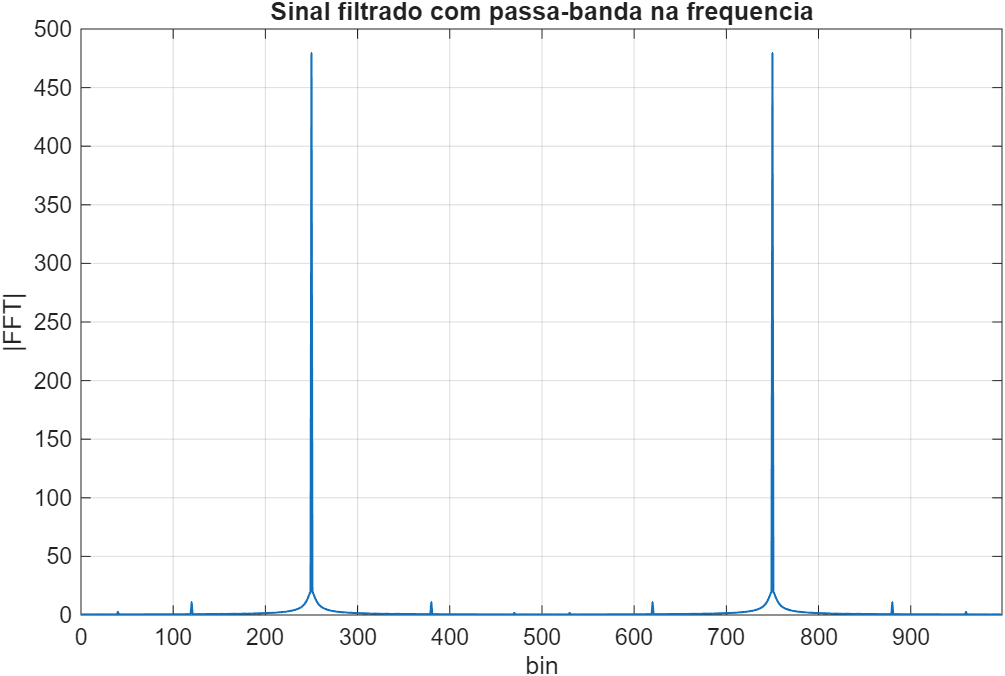
\includegraphics[width=0.8\linewidth]{figs/f4_bp_freq.png}
\caption{Sinal filtrado com o passa-banda na frequ\^encia: isola praticamente
apenas a componente de 250~Hz.}
\end{figure}

\begin{figure}[H]
\centering
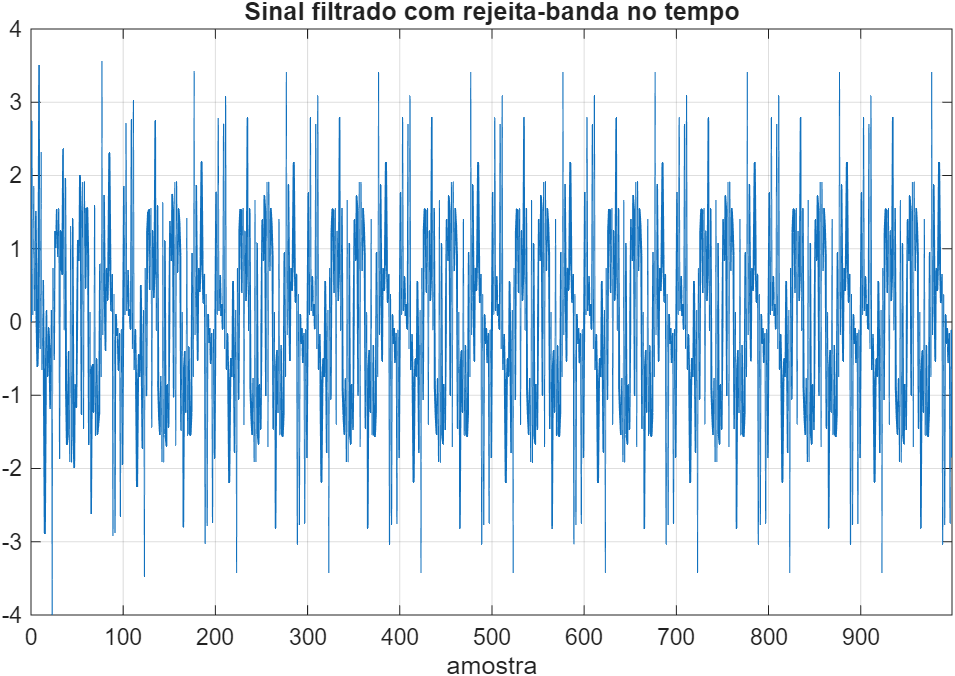
\includegraphics[width=0.8\linewidth]{figs/f4_br_tempo.png}
\caption{Sinal filtrado com o rejeita-banda (centrado em 250~Hz) no tempo.}
\end{figure}

\begin{figure}[H]
\centering
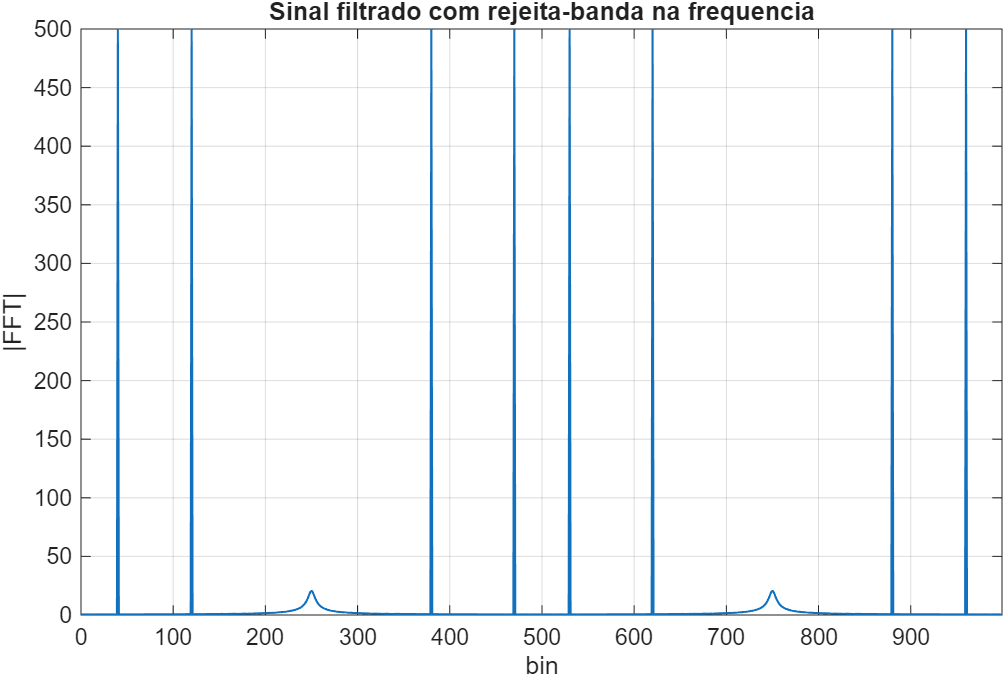
\includegraphics[width=0.8\linewidth]{figs/f4_br_freq.png}
\caption{Sinal filtrado com o rejeita-banda na frequ\^encia: elimina a raia de
250~Hz e preserva as demais quatro componentes.}
\end{figure}

O passa-banda isola praticamente apenas a componente de 250~Hz (no tempo, o sinal
filtrado tende a uma \'unica senoide ap\'os o transit\'orio inicial). J\'a o
rejeita-banda elimina a raia de 250~Hz e preserva as demais quatro componentes,
confirmando o comportamento esperado.

% ============================ ITEM 5 ============================
\section{Processamento de Som}
\textbf{Enunciado:} ``Processamento de Som (em sala, se poss\'ivel use fone de
ouvido). A este sinal, adicionamos um ru\'ido `branco' apenas com as altas
frequ\^encias, que n\~ao influencia as frequ\^encias do sinal do \'audio. E,
adicionalmente, um ru\'ido com v\'arias frequ\^encias pr\'oximas entre si, em um
local n\~ao ocupado pelo espectro do \'audio gravado. Ap\'os a inclus\~ao dos
ru\'idos, reverteu-se o espectro do sinal, como ocorre na opera\c{c}\~ao de
modula\c{c}\~ao (Equa\c{c}\~ao~1) com o uso de uma portadora $f_0$, com a
m\'axima frequ\^encia poss\'ivel para o tamanho do vetor gravado.''
\begin{equation}
x(t)\cos(2\pi f_0 t) \;\longleftrightarrow\;
\tfrac{1}{2}\big[X(f-f_0) + X(f+f_0)\big]
\end{equation}
\textbf{(continua\c{c}\~ao do enunciado):} ``Agora, de posse dos conhecimentos
adquiridos na disciplina, demodule o sinal e filtre os ru\'idos. Encontrando um
sinal o mais parecido poss\'ivel com o sinal original mostrado na Figura~1.
Dica: utilize um filtro passa baixas WindowSinc e um corta faixa Banda Estreita
(neste pode ser preciso filtrar mais de uma vez)! Qual a frase demodulada e
filtrada obtida? Gere um relat\'orio explicando detalhadamente a tomada de
decis\~ao e os procedimentos usados para demodular o sinal e isola-lo do
ru\'ido. Colocando todos os c\'odigos MATLAB e resultados obtidos.''

\vspace{0.3cm}
O arquivo \texttt{SinalRuidoModulado1s2026.mat} cont\'em a vari\'avel
\texttt{sinalModulado}, com 200.000 amostras adquiridas a $F_s = 40$~kHz (5
segundos). Sobre o sinal de voz original foram adicionados um ru\'ido branco
apenas nas altas frequ\^encias e um ru\'ido de banda estreita (v\'arias
frequ\^encias pr\'oximas) em uma regi\~ao n\~ao ocupada pela voz. Por fim, todo o
espectro foi revertido pela opera\c{c}\~ao de modula\c{c}\~ao da Equa\c{c}\~ao~1,
com portadora $f_0$ igual \`a m\'axima frequ\^encia poss\'ivel (Nyquist).

\begin{figure}[H]
\centering
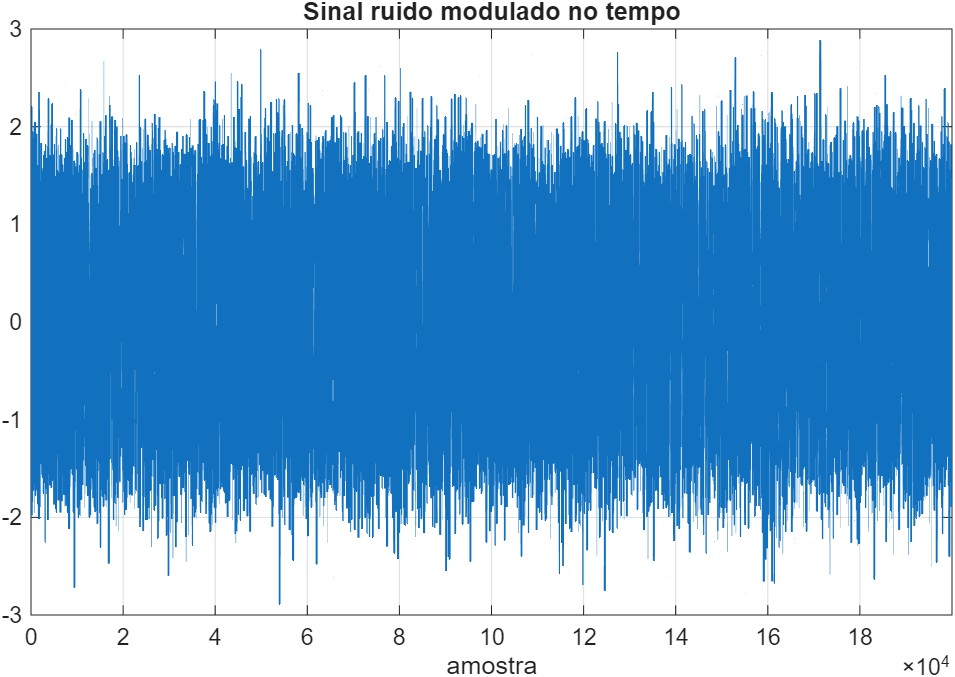
\includegraphics[width=0.8\linewidth]{figs/f5_modulado_tempo.png}
\caption{Sinal recebido (ru\'ido modulado) no tempo.}
\end{figure}

\begin{figure}[H]
\centering
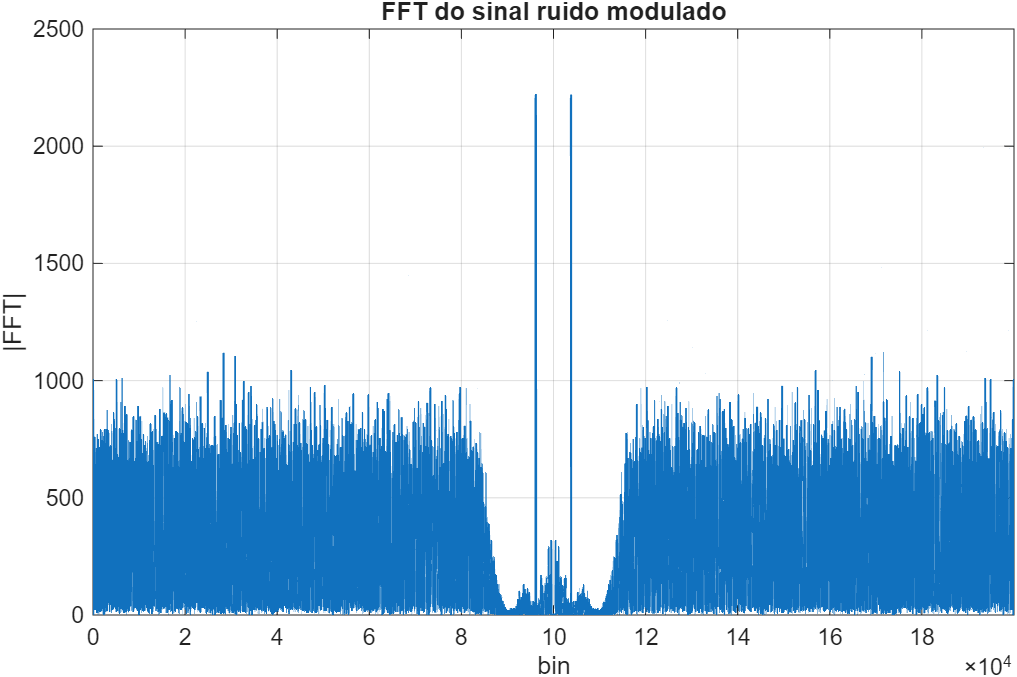
\includegraphics[width=0.8\linewidth]{figs/f5_modulado_freq.png}
\caption{Sinal recebido (ru\'ido modulado) na frequ\^encia. O espectro \'e dominado
pelo ru\'ido branco que ocupa quase toda a faixa.}
\end{figure}

\subsection*{Estrat\'egia de recupera\c{c}\~ao}
A recupera\c{c}\~ao foi dividida em tr\^es etapas: (i) demodula\c{c}\~ao espectral
para trazer a voz de volta \`as baixas frequ\^encias; (ii) filtragem passa-baixas
WindowSinc para eliminar o ru\'ido branco de alta frequ\^encia; e (iii)
rejei\c{c}\~ao de banda estreita, em cascata, para suprimir o tom interferente.

\subsection*{Demodula\c{c}\~ao espectral}
Como a invers\~ao do espectro foi feita com portadora na frequ\^encia de Nyquist
($f_0 = F_s/2 = 20$~kHz), a opera\c{c}\~ao \'e a sua pr\'opria inversa. Basta
multiplicar o sinal, amostra a amostra, por $\cos(\pi n) = (-1)^n$. Isso desloca
todo o espectro de volta, recolocando a informa\c{c}\~ao de \'audio (que estava nas
altas frequ\^encias) na faixa aud\'ivel e enviando o ru\'ido branco, que estava
sobre o \'audio, para a extremidade superior do espectro.

\begin{figure}[H]
\centering
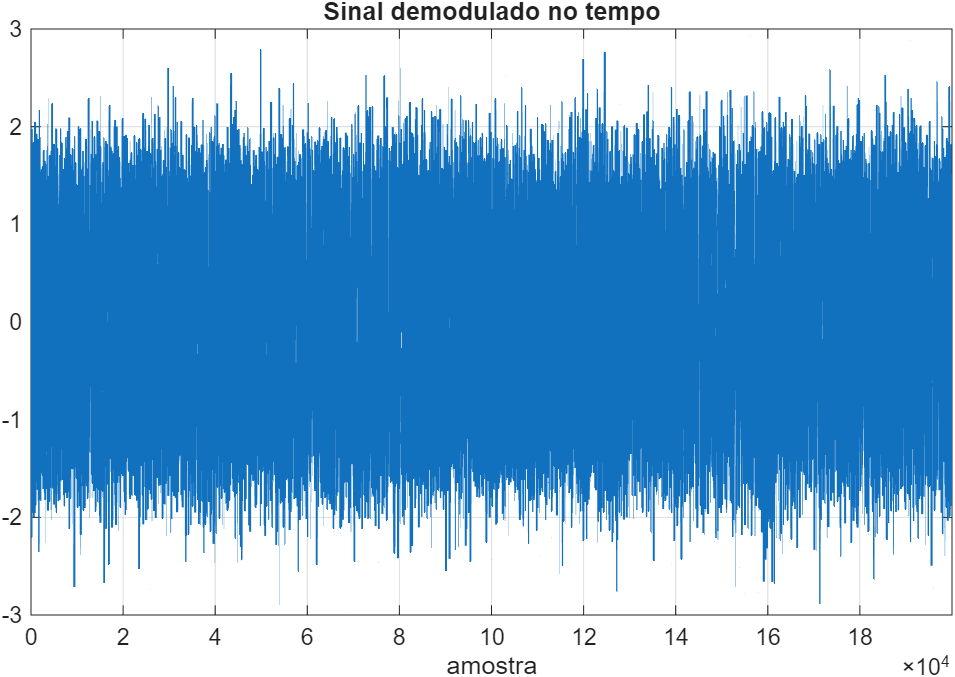
\includegraphics[width=0.8\linewidth]{figs/f5_demod_tempo.png}
\caption{Sinal ap\'os a demodula\c{c}\~ao por $\cos(\pi n)$, no tempo.}
\end{figure}

\begin{figure}[H]
\centering
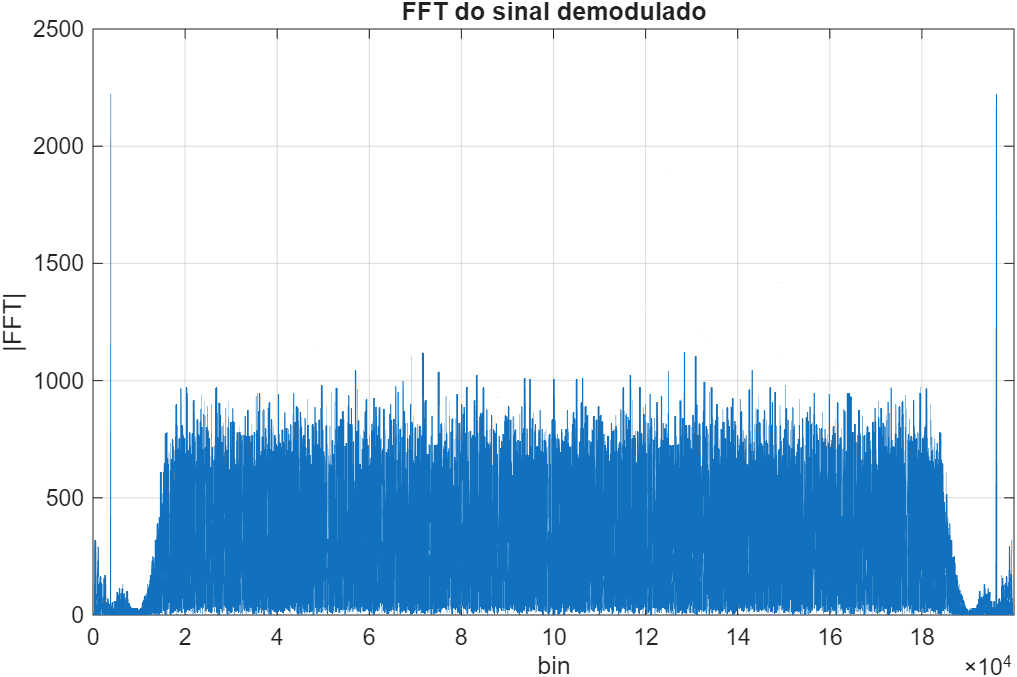
\includegraphics[width=0.8\linewidth]{figs/f5_demod_freq.png}
\caption{Sinal ap\'os a demodula\c{c}\~ao por $\cos(\pi n)$, na frequ\^encia. O
espectro foi revertido: o conte\'udo de voz reaparece em baixas frequ\^encias.}
\end{figure}

\subsection*{Filtragem passa-baixas (WindowSinc)}
Observando o espectro demodulado, o ru\'ido branco passa a ocupar as frequ\^encias
acima de aproximadamente 2{,}9~kHz, enquanto a voz fica abaixo disso. Aplicou-se
ent\~ao um filtro passa-baixas WindowSinc (janela de Blackman, 100 coeficientes,
frequ\^encia de corte normalizada $f_c = 0{,}075 \approx 3$~kHz). Por ter fase
linear, a convolu\c{c}\~ao preserva a integridade temporal da voz; o atraso de
grupo foi compensado no recorte do sinal.

\lstinputlisting[caption={WindowSinc passa-baixas (janela de Blackman) usado no item 5.}]{codigo_matlab/FWSPB.m}

\begin{figure}[H]
\centering
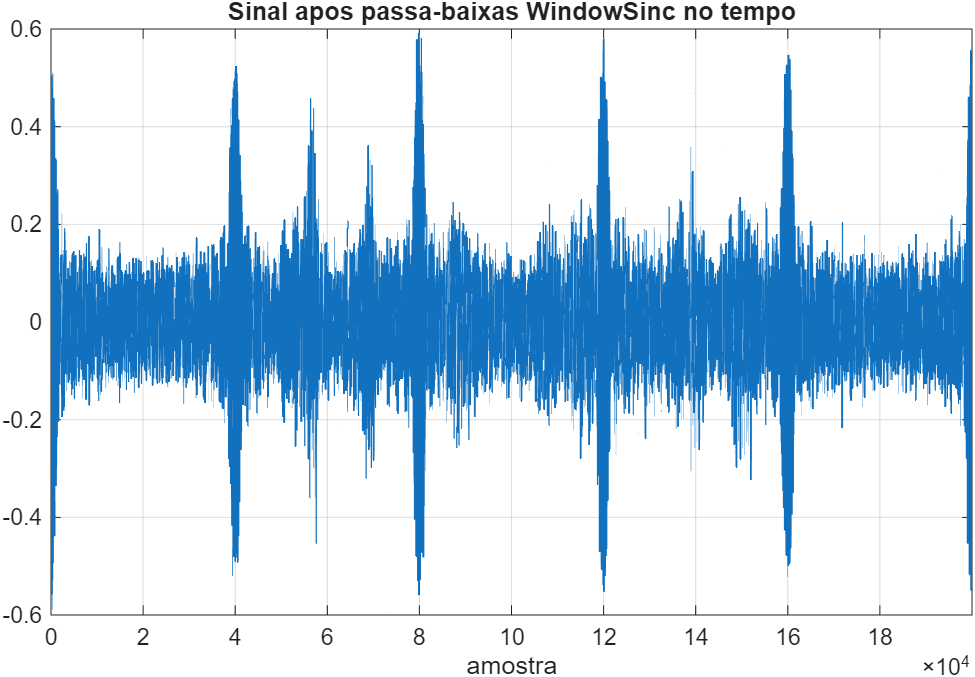
\includegraphics[width=0.8\linewidth]{figs/f5_lp_tempo.png}
\caption{Sinal ap\'os o passa-baixas WindowSinc, no tempo.}
\end{figure}

\begin{figure}[H]
\centering
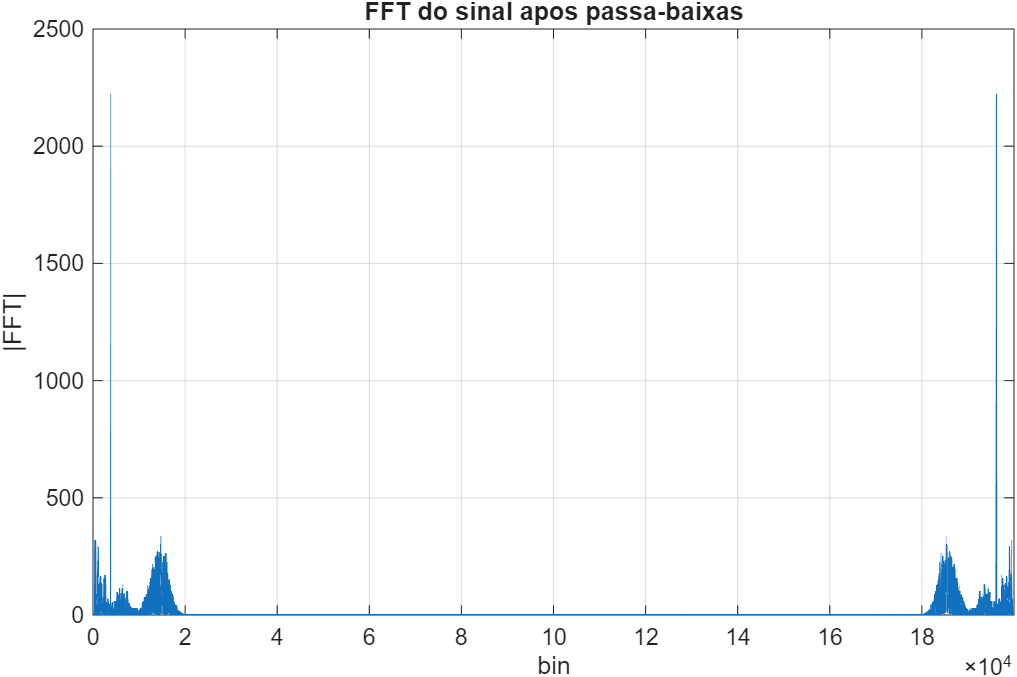
\includegraphics[width=0.8\linewidth]{figs/f5_lp_freq.png}
\caption{Sinal ap\'os o passa-baixas WindowSinc, na frequ\^encia. O ru\'ido branco
de alta frequ\^encia foi praticamente eliminado, restando a voz e um tom estreito.}
\end{figure}

\subsection*{Rejei\c{c}\~ao do tom de banda estreita}
Mesmo ap\'os o passa-baixas, persiste um tom intenso e estreito em torno de
766~Hz (frequ\^encia normalizada $\approx 0{,}0192$), correspondente ao ru\'ido de
``v\'arias frequ\^encias pr\'oximas''. Para suprimi-lo sem danificar a voz,
usou-se um filtro rejeita-banda de banda muito estreita ($BW = 0{,}0008$)
centrado nessa frequ\^encia, aplicado \textbf{tr\^es vezes em cascata}. Cada
passagem aprofunda o entalhe e soma a sua atenua\c{c}\~ao, produzindo uma
rejei\c{c}\~ao profunda do tom sem a necessidade de um filtro de ordem
excessivamente elevada.

\begin{figure}[H]
\centering
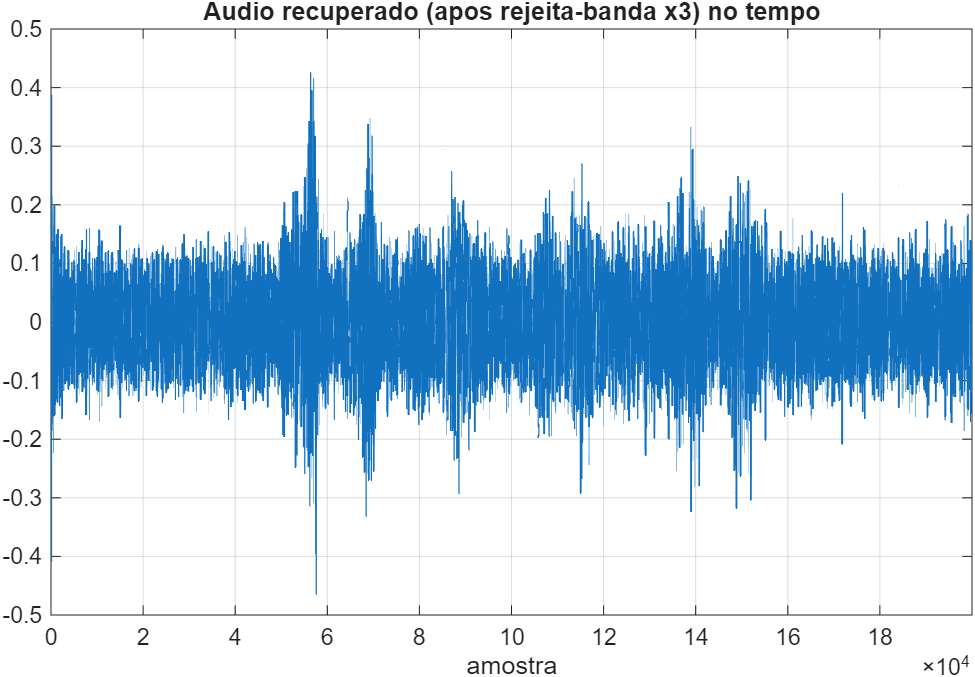
\includegraphics[width=0.8\linewidth]{figs/f5_final_tempo.png}
\caption{\'Audio recuperado (ap\'os demodula\c{c}\~ao, passa-baixas e
rejeita-banda em cascata) no tempo. Os surtos de amplitude correspondem \`as
s\'ilabas da frase falada.}
\end{figure}

\begin{figure}[H]
\centering
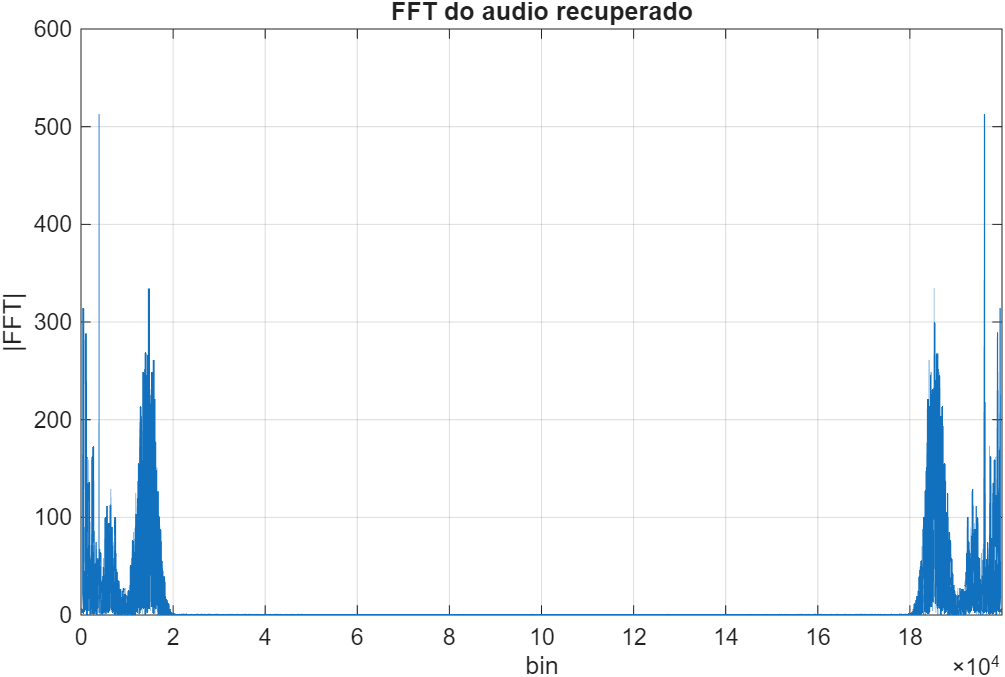
\includegraphics[width=0.8\linewidth]{figs/f5_final_freq.png}
\caption{\'Audio recuperado na frequ\^encia: a voz concentra-se nas baixas
frequ\^encias e o tom interferente em 766~Hz foi praticamente eliminado.}
\end{figure}

O c\'odigo completo do item 5 \'e apresentado a seguir.

\lstinputlisting[caption={Rotina de demodula\c{c}\~ao e filtragem do som (item 5).}]{codigo_matlab/Pratica5_item5_som.m}

\subsection*{Frase obtida}
Ap\'os a demodula\c{c}\~ao e a filtragem, o sinal recuperado foi salvo em
\texttt{sinal\_recuperado.mat} e \texttt{sinal\_recuperado.wav}. A frase
demodulada e filtrada obtida foi:
\begin{quote}
\textbf{``Ser\'a que o Hexa vem ou vamos ensacar a viola?''}
\end{quote}

% ============================ CONCLUSAO ============================
\section{Conclus\~ao}
A pr\'atica consolidou os conceitos fundamentais dos filtros IIR. A
implementa\c{c}\~ao dos filtros de p\'olo simples permitiu observar diretamente a
rela\c{c}\~ao entre a constante $r$, a frequ\^encia de corte e o decaimento da
resposta ao impulso, bem como o comportamento suave das curvas de ganho e fase
de um sistema de primeira ordem. Os filtros de banda
estreita, de segunda ordem, evidenciaram o papel do par\^ametro $BW$ no
posicionamento dos p\'olos e na sele\c{c}\~ao (ou rejei\c{c}\~ao) de uma faixa
estreita do espectro.

A etapa de processamento de som foi a mais completa: combinando demodula\c{c}\~ao
espectral, um filtro passa-baixas WindowSinc de fase linear e um rejeita-banda
estreito aplicado em cascata, foi poss\'ivel reverter a invers\~ao do espectro,
remover o ru\'ido branco de alta frequ\^encia e suprimir o tom interferente,
recuperando a mensagem de voz original de forma intelig\'ivel. O exerc\'icio
refor\c{c}ou a import\^ancia de identificar corretamente, no dom\'inio da
frequ\^encia, as faixas de interesse e de projetar o filtro adequado a cada etapa
do processamento.

\end{document}
